\documentclass[template=tabling,81pt,headonall]{azmoon}
\usepackage{xepersian}
\usepackage{amsfonts}
\usepackage{graphicx}
\graphicspath{ {./images/} }
\settextfont{Yas}
\setdigitfont{A Iranian Sans}

\printanswers

\teacher{آقای معلوم نیست}
\teachertitle{دبیر}
\city{مشهد}
\schooltitle{دبیرستان}
\school{معلوم نیست}
\grade{هشتم}
\branch{معلوم نیست}
\topic{ریاضی}
\examdate{به سوی بینهایت و فراتر از آن}
\answertime{70 دقیقه}
\begin{document}
	\begin{questions}
		\nointerlineskip%
		\vskip-\baselineskip
		
		\question{%
		در فرایند پیدا کردن عددهای اول بین ۲۰ و ۴۰، ب.م.م. دوومین عدد که در مضرب ۲ خط می‌خورد و ششمین عددی که از مضرب ۳ خط می‌خورد کدام است.
			\begin{fourchoice}
				\choice{۳}
				\choice{۲}
				\choice{۵}
				\choice{۷}
			\end{fourchoice}
		}
		\question{
		در شکل زیر مقدار  $O+A_1$ کدام است؟ (  $C_2=40^{O}$   ،   $C_1$  و $C_2$ متمم)
			
		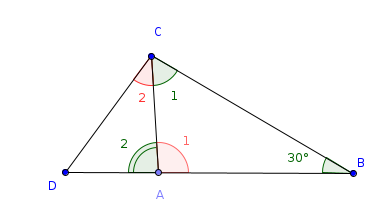
\includegraphics[scale = 0.35]{image_2}
		\begin{fourchoice}
				\choice{130}
				\choice{150}
				\choice{160}
				\choice{140}
		\end{fourchoice}
		}
		\question{%
		مقدار ساده شده عبارت
		$3(2x+a)-2(3a+x)$
		در کدام گزینه آمده است.
			\begin{fourchoice}[2]
				\choice{$-8x+9a$}
				\choice{$4x$}
				\choice{$8x-9a$}
				\choice{$-8x+9a$}
			\end{fourchoice}
		}
		\question{
			مساحت مستطیل به طول 
			$(2x+y)$
			و عرض
			$(2y+3x)$
			کدام است؟
			\begin{fourchoice}[2]
				\choice{$2(x^2+y^2+xy)$}
				\choice{$4(x^2-y^2+2xy)$}
   				\choice{$2(2x^2+y^2+3xy)$}
				\choice{$4(x^2+y^2+xy)$}
			\end{fourchoice}

		}
		\question{
			مقدار 
			x
			 در معادله 
			$\dfrac{1}{2}x-\dfrac{4}{5}=\dfrac{2}{3}x$
			کدام است.
			\begin{fourchoice}
				\choice{$-\dfrac{24}{5}$}
				\choice{$\dfrac{24}{5}$}
				\choice{$\dfrac{24}{35}$}
				\choice{$-\dfrac{24}{35}$}
			\end{fourchoice}

		}
		\question{
			اگر
			$3x-3=7x-2x+5$
			مقدار
			$x+4$
			کدام است؟
			\\

			\begin{fourchoice}
				\choice{-4}
				\choice{0}
				\choice{-1}
				\choice{+1}
			\end{fourchoice}
		}
		\question{
			پنج برابر عددی منهای ۳ مساوی با سه برابر همان عدد به اضافه ۷ است آن عدد را بیابید.
			\\
			\begin{fourchoice}
				\choice{5}
				\choice{10}
				\choice{2}
				\choice{$\frac{1}{2}$}
		\end{fourchoice}
		}
		\question{
			اگر
			$b=i, a = 2i-j$
			مختصات بردار 
			$\overrightarrow{x} $
			که به صورت 
			$\overrightarrow{x}=3a+4b $
			است، کدام است؟
			\\
			
			
			\begin{fourchoice}[2]
				\choice{$6i-3j$}
				\choice{$4i+3j$}
				\choice{$i+j$}
				\choice{$10i-3j$}
		\end{fourchoice}
		}
		\question{
بردار مختصاد یک رباط طوری طراحی شده است که از مبدأ مختصات یک واحد به راست و یک واحد به بالا حرکت می‌کند و یک مکث ی‌کند و همین روند را تکرار می‌کند. اگر این رباط در مکث ششم در نقطه $C$ باشد مقدار $5C+3j$ کدام است؟
\\
		\begin{fourchoice}
			\choice{$6i+6j$}
			\choice{$30j+23j$}
			\choice{$33i+30j$}
			\choice{$20i+23j$}
	\end{fourchoice}
		}
		\question{
مقدار $x$ را طوری بدست آورید که:
\\
$2x^2-2x(x+3) = 4+7(x+5)$
\\
		\begin{fourchoice}
			\choice{$-\frac{9}{13}$}
			\choice{$\frac{5}{13}$}
			\choice{$\frac{9}{1}$}
			\choice{$-\frac{6}{5}$}
	\end{fourchoice}
		}
		\question{
		اگر یک چند ضلعی منتظم از ۶ مثلث متساوی الاضلاع تشکیل شده باشد شکل حاصل چند ضلعی است و اندازه زاویه داخلی آن چند درجه است؟
		\\
		\begin{fourchoice}[2]
			\choice{8ضلعی و 135 درجه}
			\choice{6ضلعی و 120 درجه}
			\choice{4ضلعی و 90 درجه}
			\choice{5 ضلعی و 108 درجه}
			

		\end{fourchoice}


		}
		\question{
		در شکل زیر پاره خط
		$CD$
		را از روی خطر $BE$موازی خط
		$BA$
		رسم کرده‌ایم. اندازه زاویه $\widehat{ADC}$ را بدست آورید. 

		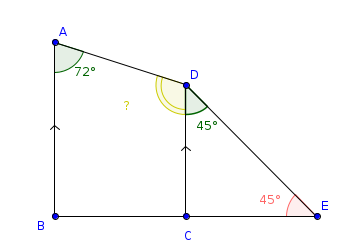
\includegraphics[scale = 0.35]{image_12}
		
		\begin{fourchoice}
			\choice{$\frac{153}{2}$}
			\choice{153}
			\choice{108}
			\choice{$\frac{108}{2}$}
		\end{fourchoice}
		}
		\question{
			مقدار
			$x-y$
			کدام است؟

			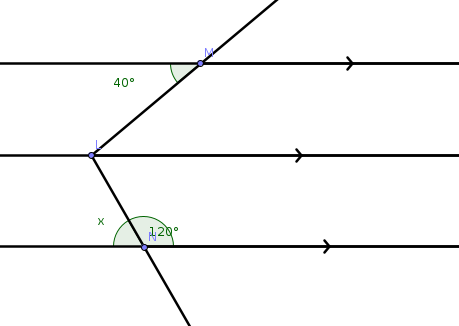
\includegraphics[scale = 0.35]{image_13}
			\\
			\begin{fourchoice}
				\choice{60}
				\choice{120}
				\choice{100}
				\choice{140}
			\end{fourchoice}
		}
			
		\question{
			در یک ۵ ضلعی منتظم مقدار یک زاویه خارجی برابر 
		$2x+10$
			است. مقدار$x$
			کدام است؟

			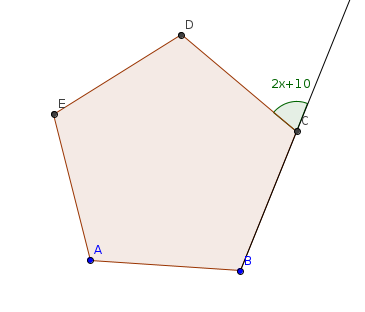
\includegraphics[scale = 0.35]{image_14}
			
			\begin{fourchoice}
				\choice{62}
				\choice{31}
				\choice{41}
				\choice{81}
			\end{fourchoice}
		}
		\question{
			بردار
			$\overrightarrow{a}=3i+2j $
			و
			$\overrightarrow{b}=4i-3j $
			را داریم. بردارهای 
			$a,b,c$
			مطابق شکل زیر به ظاهر یک مثلث دیده می‌شوند. بردار 
			$\overrightarrow{c} $
			 کدام یک از گزینه‌های زیر است؟

			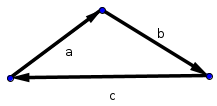
\includegraphics[scale = 0.35]{image_15}
			\begin{fourchoice}
				\choice{$7i-j$}
				\choice{$-7i+j$}
				\choice{$i-5j$}
				\choice{$-i+5j$}
			\end{fourchoice}
		}
		\question{
		درباره روابط بین مجموعه‌های اعداد صحیح
			$(\mathbb{Z})$ 
		گویا
		$(\mathbb{Q})$
		و طبیعی
		$(\mathbb{N})$
		کدام یک از گزینه‌های زیر برقرار است؟
		\begin{fourchoice}
				\choice{$\mathbb{N} \subseteq \mathbb{Q} \subseteq \mathbb{Z}$}
				\choice{$\mathbb{N} \subseteq \mathbb{Z} \subseteq \mathbb{Q}$}
				\choice{$\mathbb{Z} \subseteq \mathbb{N} \subseteq \mathbb{Q}$}
				\choice{$\mathbb{Q} \subseteq \mathbb{N} \subseteq \mathbb{Z}$}
			\end{fourchoice}
		}
		\question{
		حاصل کدام یک از گزینه‌های زیر گویا است؟
		
		\begin{fourchoice}
			\choice{$\frac{2\pi}{3}\times \frac{3}{4}$}
			\choice{$\frac{5\times \sqrt{3}}{\sqrt{7}}$}
			\choice{$\sqrt{\frac{4}{3} \times 2}$}
			\choice{$\sqrt{\frac{5 \times 7 \times 8}{7\times4}}$}
		
			\end{fourchoice}
		}
		\question{
		حاصل عبارت
		$\frac{4}{3} \times \frac{39}{4}$
		کدام است؟
		\begin{fourchoice}
			\choice{$13$}
			\choice{$\frac{133}{12}$}
			\choice{$\frac{43}{12}$}
			\choice{$\frac{43}{7}$}
		\end{fourchoice}
		}
		\question{
		حاصل عبارت
		$-\frac{2}{3} + \frac{6}{7}$
		چند است؟
		\begin{fourchoice}
			\choice{$\frac{4}{21}$}
			\choice{-$\frac{4}{21}$}
			\choice{$\frac{8}{10}$}
			\choice{$\frac{4}{10}$}
		\end{fourchoice}
		}
		\question{
		حاصل عبارت
		$\frac{\frac{2}{3} + \frac{4}{3}}{\frac{1}{5}}$
		برابر کدام یک از گزینه‌های زیر است؟
		\\
		\begin{fourchoice}
			\choice{$\frac{5}{2}$}
			\choice{$\frac{2}{5}$}
			\choice{$10$}
			\choice{$\frac{6}{3}$}
		\end{fourchoice}
		}
		\question{
		دانش‌آموزی در مسیر بدست آوردن حاصل عبارت
		$(-\frac{2}{7})\div (+\frac{4}{3})$
		دچار اشتباه شده و حاصل را
		$\frac{13}{28}$
		بدست آورده. راه حل این دانش‌آموز در زیر آمده است:
		\\
		$(-\frac{2}{7})\div(+\frac{4}{3}) = -(\frac{2}{7})\div(\frac{4}{3}) = -(\frac{2}{7})\times (\frac{3}{4}) = \frac{-8+21}{28} = \frac{13}{28}$
		\\
		کدام گزینه به اشتباه دانش‌آموز اشاره می‌کند؟
		\begin{fourchoice}[1]
			\choice{بعد از قسمت 
				$-(\frac{2}{7})\div (\frac{4}{3})$
				به اشتباه جای صورت و مخرج کسر
				$\frac{4}{3}$
				را جا‌به‌جا نوشته اند.}
			\choice{در ضرب دو کسر$\frac{3}{4}$ و $-\frac{2}{7}$ اشتباه شده است و به اشتباه دو کسر با هم جمع شده است.}
			\choice{علامت منفی قبل $-8+21$ فراموش شده و حاصل عبارت مثبت نوشته شده.}
			\choice{عدد ۲۱ و ۲۸ در 
			$\frac{-8+21}{28}$
			با هم ساده می‌شدند و می‌داشتیم
			$\frac{-8+3}{4}=\frac{-5}{4}$}
		\end{fourchoice}
		}
		\question{
		دانش‌آموزی در محاسبه حاصل عبارت
		$-(\frac{3}{4})\times (-\frac{8}{24})$
		اشتباه کرده و حاصل را
		$\frac{1}{4}$
		به دست آورده. مسیر حل او به شکل زیر است:
		\\
		$(-\frac{3}{4})\times(-\frac{8}{24}) = +(\frac{3}{4})\times(\frac{8}{24}) = +(\frac{3}{4})\times (\frac{1}{3}) = +(\frac{1}{4})\times 1 = \frac{1}{4}$
		\\
		کدام گزینه به اشتباه دانش‌آموز اشاره می‌کند؟
		\begin{fourchoice}[1]
			\choice{در شروع کار علامت «-» را فراموش کرده.}
			\choice{در ساده کردن عبارت $+(\frac{3}{4})\times (\frac{8}{24})$
			باید ۳ و ۲۴ را باهم ساده می‌کرد و به عبارت
			$\frac{1}{4}\times\frac{8}{8}$
			می‌رسید و بعد ادامه می‌داد.}
			\choice{ابتدا باید برای دو کسر $(\frac{3}{4})$ و 
			$\frac{8}{24}$
			مخرج مشترک ۲۴ را انتخاب می‌کرد و بعد ادامه می‌داد.}
			\choice{دانش‌آموز اشتباهی نکرده.}
		\end{fourchoice}
		}
		\question{
			تعدادی مکعب
			$1\times1\times1$
			داریم که می‌خواهیم با در کنار هم چیدن این مکعب‌ها یک مکعب مستطیل (تو پر) بدست بیاید که اضلاعش حتما بیشتر از یک باشد. مثلا مکعب مستطیل 
			$3\times4\times1$
			نمی‌تواند باشد، چون یک ضلعش «۱» است. کدام یک از گزینه‌ها می‌تواند تعداد این مکعب‌ها باشد تا بتوانیم به همچین چینشی برسیم؟
			\begin{fourchoice}
				\choice{49}
				\choice{30}
				\choice{7}
				\choice{21}
			\end{fourchoice}
			}
		\question{
		ماشین اصغر در هر ۱۰۰ کیلومتر که مسافت طی می‌کند 		
		$6.7$
		لیتر بنزین مصرف می‌کند. اصغر برای احطیات بک ۴ لیتری بنزین در ماشین دارد. در صورت خالی شدن باک ماشین اصغر تا چند کیلومتر دیگر را می‌تواند به کمک آن ۴ لیتری برود؟
		\begin{fourchoice}
					\choice{$59.70$}
					\choice{$5.97$}
					\choice{$67.50$}
					\choice{$6.75$}
				\end{fourchoice}
		}
		\question{
			در محوطه یک مجموعه آموزشی مسجد با ظاهر هشت ضلعی منتظم طراحی شده امتداد یکی از دیوارهای مسجد با ساختمان خوابگاه این مجموعه زاویه
			$15^{\circ} $
			می‌سازد. کسی داخل خوابگاه می‌خواهد رو بهه قبله بایستد. بعد از ایستادن روبه دیوار مشخص شده چند درجه باید به سمت چپ بچرخد؟
		
		
			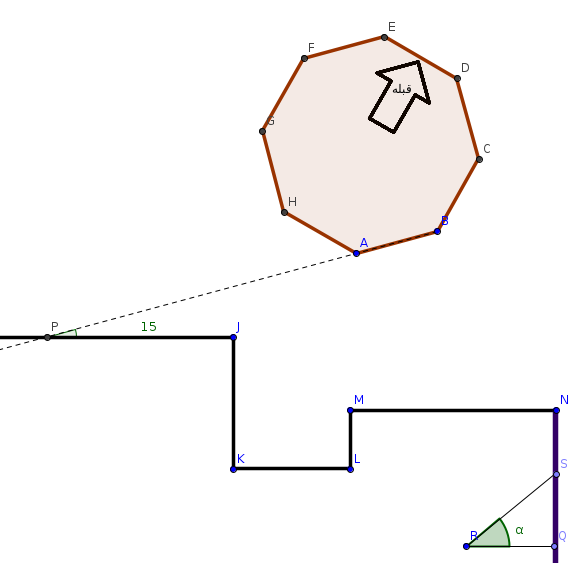
\includegraphics[scale = 0.45]{image_25}
		\begin{fourchoice}
				\choice{$37.5$}
				\choice{$33.75$}
				\choice{$27.5$}
				\choice{$35.5$}
		\end{fourchoice}
		}
		
	\end{questions}
\end{document}